% Harus dimuat terlebih dahulu, digunakan agar file PDF memiliki format karakter yang benar.
% Untuk informasi lebih lanjut, lihat https://ctan.org/pkg/cmap.
\RequirePackage{cmap}

% Format dokumen sebagai paper konferensi menggunakan aturan IEEEtran terbaru (v1.8b).
% Untuk informasi lebih lanjut, lihat http://www.michaelshell.org/tex/ieeetran/.
\documentclass[conference]{IEEEtran}[2015/08/26]

% Format encoding font dan input menjadi 8-bit UTF-8.
\usepackage[T1]{fontenc}
\usepackage[utf8]{inputenc}

% Format bahasa menjadi bahasa german dan inggris.
\usepackage[indonesian]{babel}

% Digunakan untuk tujuan demonstrasi.
\usepackage{mwe}

% Digunakan untuk menampilkan font dengan style yang lebih baik.
\usepackage[zerostyle=b,scaled=.75]{newtxtt}

% Digunakan untuk menampilkan tabel dengan style yang lebih baik.
\usepackage{booktabs}

% Digunakan untuk menampilkan gambar pada dokumen.
\usepackage{graphicx}

% Digunakan untuk menampilkan potongan kode.
\usepackage{listings}
\lstset{
  basicstyle=\ttfamily,
  columns=fixed,
  basewidth=.5em,
  xleftmargin=0.5cm,
  captionpos=b
}

% Digunakan agar backticks (`) dapat dirender pada PDF.
% Untuk informasi lebih lanjut, lihat https://tex.stackexchange.com/a/341057/9075.
\usepackage{upquote}

% Digunakan untuk menyeimbangkan bagian akhir dokumen dengan dua kolom.
\usepackage{balance}

% Digunakan untuk menampilkan pustaka.
\usepackage[square,comma,numbers,sort&compress]{natbib}

% Mengubah format ukuran teks pada natbib.
\renewcommand{\bibfont}{\normalfont\footnotesize}

% Menambah nama penulis ketika menggunakan perintah \citet.
% Untuk informasi lebih lanjut, lihat https://tex.stackexchange.com/a/76075/9075.
\usepackage{etoolbox}
\makeatletter
\patchcmd{\NAT@test}{\else \NAT@nm}{\else \NAT@hyper@{\NAT@nm}}{}{}
\makeatother

% Digunakan untuk melakukan linewrap pada pustaka dengan url yang panjang
% jika terdapat hyphens
\usepackage[hyphens]{url}

% Digunakan untuk menambah hyperlink pada referensi.
\usepackage{hyperref}

% Menonaktifkan warna dan bookmark pada hyperref.
\hypersetup{hidelinks,
  colorlinks=true,
  allcolors=black,
  pdfstartview=Fit,
  breaklinks=true
}

% Digunakan untuk membenarkan hyperref pada gambar.
\usepackage[all]{hypcap}

% Digunakan untuk menampilkan beberapa gambar
\usepackage[caption=false,font=footnotesize]{subfig}

\usepackage{stfloats}

% Tambahkan format tanda hubung yang benar di sini
\hyphenation{
  ro-ket
  me-ngem-bang-kan
  per-hi-tu-ngan
}

\begin{document}

  % Ubah kalimat berikut sesuai dengan judul penelitian.
\title{Perancangan Sistem Kontrol Motor Kursi Roda Secara Nirkabel Berbasis ESP32}

% Ubah kalimat-kalimat berikut sesuai dengan nama, institusi, alamat dan kontak penulis.
\author{
  \IEEEauthorblockN{I Putu Haris Setiadi Ekatama}
  \IEEEauthorblockA{Departemen Teknik Komputer\\
    Fakultas Teknologi Elektro dan Informatika Cerdas\\
    Institut Teknologi Sepuluh Nopember\\
    Surabaya, Indonesia 60111\\
    \href{mailto:haris.ekatama@gmail.com}{haris.ekatama@gmail.com}}

  \and
  \IEEEauthorblockN{Dr. Eko Mulyanto Yuniarno, S.T., M.T.}
  \IEEEauthorblockA{Departemen Teknik Komputer\\
    Fakultas Teknologi Elektro dan Informatika Cerdas\\
    Institut Teknologi Sepuluh Nopember\\
    Surabaya, Indonesia 60111\\
    \href{mailto:ekomulyanto@ee.its.ac.id}{ekomulyanto@ee.its.ac.id}}
}

% Digunakan untuk menampilkan judul dan deskripsi penulis.
\maketitle

  % Mengubah keterangan `Abstract` ke bahasa indonesia.
% Hapus bagian ini untuk mengembalikan ke format awal.
\renewcommand\abstractname{Abstract}

\begin{abstract}

  % Ubah paragraf berikut sesuai dengan abstrak dari penelitian.
  \emph{Paralysis is a condition where a person experiences a weakening of the functions in their body parts, causing them to lack energy or be unable to move their limbs as they should. There are several conditions that can lead to paralysis, ranging from diseases such as stroke to accidents. Individuals experiencing paralysis often face challenges in their daily mobility. They require additional tools to be able to carry out activities, one of which is a wheelchair. Electric wheelchairs controlled by a joystick have been developed to date. However, the use of a joystick may not address the issues faced by someone experiencing paralysis. This is because individuals with paralysis in their arms may struggle to control this type of electric wheelchair. In this research, a controller for an electric wheelchair has been developed that can be operated through computer vision technology, either with hand poses or head gestures. The integration of this technology can be an innovative solution to the problems being faced. Choosing ESP32 as the main microcontroller is a strategic step due to its ability to precisely control the wheelchair's motor. In addition to functioning as a motor controller, ESP32 also serves as a data receiver from the computer equipped with computer vision technology. From the test results, it is concluded that the transmission from computer vision should be analogized to 1 character letter and transmitted using WiFi. This is done because transmitting data containing 1 letter and using WiFi has the best delay time, which is 0.03499708571 seconds. Through this integration, it is expected that the motor controller can operate synergistically with the information received from the computer, creating an efficient and responsive system.}

\end{abstract}

% Mengubah keterangan `Index terms` ke bahasa indonesia.
% Hapus bagian ini untuk mengembalikan ke format awal.
\renewcommand\IEEEkeywordsname{Keywords}

\begin{IEEEkeywords}

  % Ubah kata-kata berikut sesuai dengan kata kunci dari penelitian.
  \emph{Wheelchair}, \emph{Convolutional Neural Network}, \emph{Mediapipe}, \emph{ESP32}, \emph{WiFi}.

\end{IEEEkeywords}


  % Ubah bagian berikut sesuai dengan konten-konten yang akan dimasukkan pada dokumen
  % Ubah judul dan label berikut sesuai dengan yang diinginkan.
\section{Pendahuluan}
\label{sec:pendahuluan}

% Ubah paragraf-paragraf pada bagian ini sesuai dengan yang diinginkan.

Menurut Kamus Besar Bahasa Indonesia, lumpuh merupakan melemahnya fungsi anggota badan sehingga tidak bertenaga atau tidak dapat digerakkan lagi sebagaimana mestinya \cite{Daring_2016}. Otot beserta tulang, saraf, serta jaringan penghubung antara otot, tulang dan saraf memiliki peran yang penting dalam mengendalikan gerak tubuh manusia. Apabila salah satu jaringan mengalami gangguan makan akan terjadi kelumpulan, baik kelumpuhan sementara maupun kelumpuhan permanen.

Terdapat beberapa kondisi yang dapat mengakibatkan kelumpuhan, seperti penyakit stroke yang dapat menyebabkan kelumpuhan pada salah satu sisi wajah, lengan serta tungkai, \emph{Bell's Palsy} yang dapat menyebabkan kelumpuhan pada salah satu sisi wajah tanpa disertai kelumpuhan pada anggota tubuh yang lain, cedera otak yang dapat memicu kelumpuhan pada setiap bagian tubuh sesuai bagian otak yang rusak, polio yang menyebabkan kelumpuhan pada lengan, tungkai, serta otot pernapasan, dan masih banyak kondisi yang menyebabkan kelumpuhan \cite{Pansawira_2022}.

Seseorang yang mengalami kelumpuhan sering kali mengalami permasalahan dalam hal mobilitas sehari-hari. Mereka memerlukan alat tambahan untuk dapat beraktivitas sehari-hari, salah satunya adalah kursi roda. Hingga saat ini sudah terdapat kursi roda elektrik yang dikendalikan dengan menggunakan \emph{joystick} \cite{choi2019motion}. Akan tetapi penggunaan \emph{joystick} belum dapat menjawab permasalahan dari seseorang yang mengalami kelumpuhan. Karena bagi orang yang mengalami kelumpuhan pada bagian lengan akan kekusahan dalam mengendalikan kursi roda elektrik berjenis ini.

Dalam menghadapi permasalahan kelumpuhan, sangat penting untuk mencari solusi yang dapat meningkatkan kemandirian para penderita. Salah satu pendekatan yang menjanjikan adalah memanfaatkan teknologi canggih, seperti visi komputer yang dapat diintegrasikan dengan sistem tertanam. Dengan menggabungkan kedua teknologi ini, diharapkan dapat diciptakan solusi inovatif yang memungkinkan para penderita kelumpuhan untuk tetap dapat bermobilitas secara mandiri.

Visi komputer merupakan bidang keilmuan yang memungkinkan komputer dapat "melihat" \cite{TIAN20201}. Teknologi ini menggunakan kamera untuk mengidentifikasi, melacak, hingga mengukur target untuk pemrosesan citra lebih lanjut. Visi komputer memberikan kemampuan untuk mengenali dan memahami lingkungan sekitar. Sedangkan sistem tertanam dapat diatur secara personal untuk memenuhi kebutuhan spesifik sesuai dengan permasalahan yang dihadapi. 

Integrasi teknologi ini dapat menjadi solusi inovatif terhadap permasalahan yang dihadapi. Dalam rangka mengatasi tantangan ini, penelitian akan difokuskan pada pengembangan kontroler motor yang dapat secara optimal berinteraksi dengan teknologi visi komputer. Pemilihan ESP32 sebagai mikrokontroler utama menjadi langkah strategis, karena kemampuannya dalam mengatur dengan presisi kerja motor. Tidak hanya berfungsi sebagai kontroler motor, ESP32 juga akan berperan sebagai perangkat penerima data dari komputer yang dilengkapi dengan teknologi visi komputer. Melalui integrasi ini, diharapkan bahwa kontroler motor dapat beroperasi secara sinergis dengan informasi yang diterima dari komputer dan menciptakan sebuah sistem yang efisien dan responsif. 

  % Ubah judul dan label berikut sesuai dengan yang diinginkan.
\section{Penelitian Terkait}
\label{sec:penelitianterkait}

% Ubah paragraf-paragraf pada bagian ini sesuai dengan yang diinginkan.

Beberapa penelitian lain pernah dilakukan seperti yang dirumuskan oleh \citet{newton1687} bahwa \lipsum[5]
Hasil tersebut kemudian menjadi persamaan \ref{eq:hukumpertama}.

% Contoh pembuatan persamaan ilmiah.
\begin{equation}
  \label{eq:hukumpertama}
  \sum \mathbf{F} = 0\; \Leftrightarrow\; \frac{\mathrm{d} \mathbf{v} }{\mathrm{d}t} = 0.
\end{equation}

\lipsum[6-7]

  % Ubah judul dan label berikut sesuai dengan yang diinginkan.
\section{Architecture}
\label{sec:arsitektur}

% Ubah paragraf-paragraf pada bagian ini sesuai dengan yang diinginkan.
In this study, a control device has been developed that can receive commands wirelessly from other devices such as a laptop or Jetson Nano. This subsection will detail the implementation of the device developed in this research.

Below are detailed some of the hardware and software used in this research, as follows:
\begin{enumerate}
    \item Anaconda Navigator
    \item Arduino IDE 
    \item Laptop 
    \item Jetson Nano
    \item Camera
    \item ESP32 Devkit V1
    \item 2 Motor Driver
    \item 2 DC-DC Voltage Regulator
    \item 2 DC Motor
    \item 24V Battery
\end{enumerate}

\subsection{Schematic}
\label{subsec:skematik alat}

The schematic of this device is illustrated in detail in Figure \ref{fig:Skematik Alat}. This system utilizes a camera connected to a laptop or Jetson Nano as the main device for capturing images. The workflow begins when the camera captures images of the object. These captured images are then processed by the laptop or Jetson Nano. In this system, a pre-programmed classification model plays a crucial role in interpreting the image data. The results of this classification process are crucial as they form the basis for determining the instruction codes to be implemented.

The instruction codes will then be combined with the maximum speed parameters previously set by the user. The combination of instruction codes and speed parameters will form a data package as wheelchair motion control. This data package will then be transmitted wirelessly, either via Bluetooth or WiFi, to the ESP32 Devkit V1 module.

The ESP32 plays a crucial role in controlling the wheelchair motor. The ESP32 will serve as the control center that receives the data package sent wirelessly by the user. Subsequently, the ESP32 will decode the data package and adjust the data into predefined variables. This data package decoding process will yield two main pieces of data, which will then be further processed by the ESP32.

The first variable is the direction variable, which plays a crucial role in determining the direction of movement for the wheelchair's two motors. This variable ensures that the motors move in the desired direction based on the received data. Additionally, there is the speed variable used to set the maximum speed of the motor movement.

In its implementation, there is a series of chained 'if' logics that will be detailed in the programming subsection. Simply put, this chained 'if' logic plays a crucial role in decision-making for both the direction and speed of the motors based on the received data. The result of this logic will provide triggers in the form of either 5V or 0V. This voltage will then influence the motor rotation direction.

Next, the speed variable will be used to adjust the Pulse Width Modulation (PWM) level on the motor controller. This PWM adjustment is crucial for controlling the motor rotation speed. By adjusting the PWM level, the maximum motor speed can be customized according to the requirements.

\begin{figure} [!ht] \centering
  % Nama dari file gambar yang diinputkan
  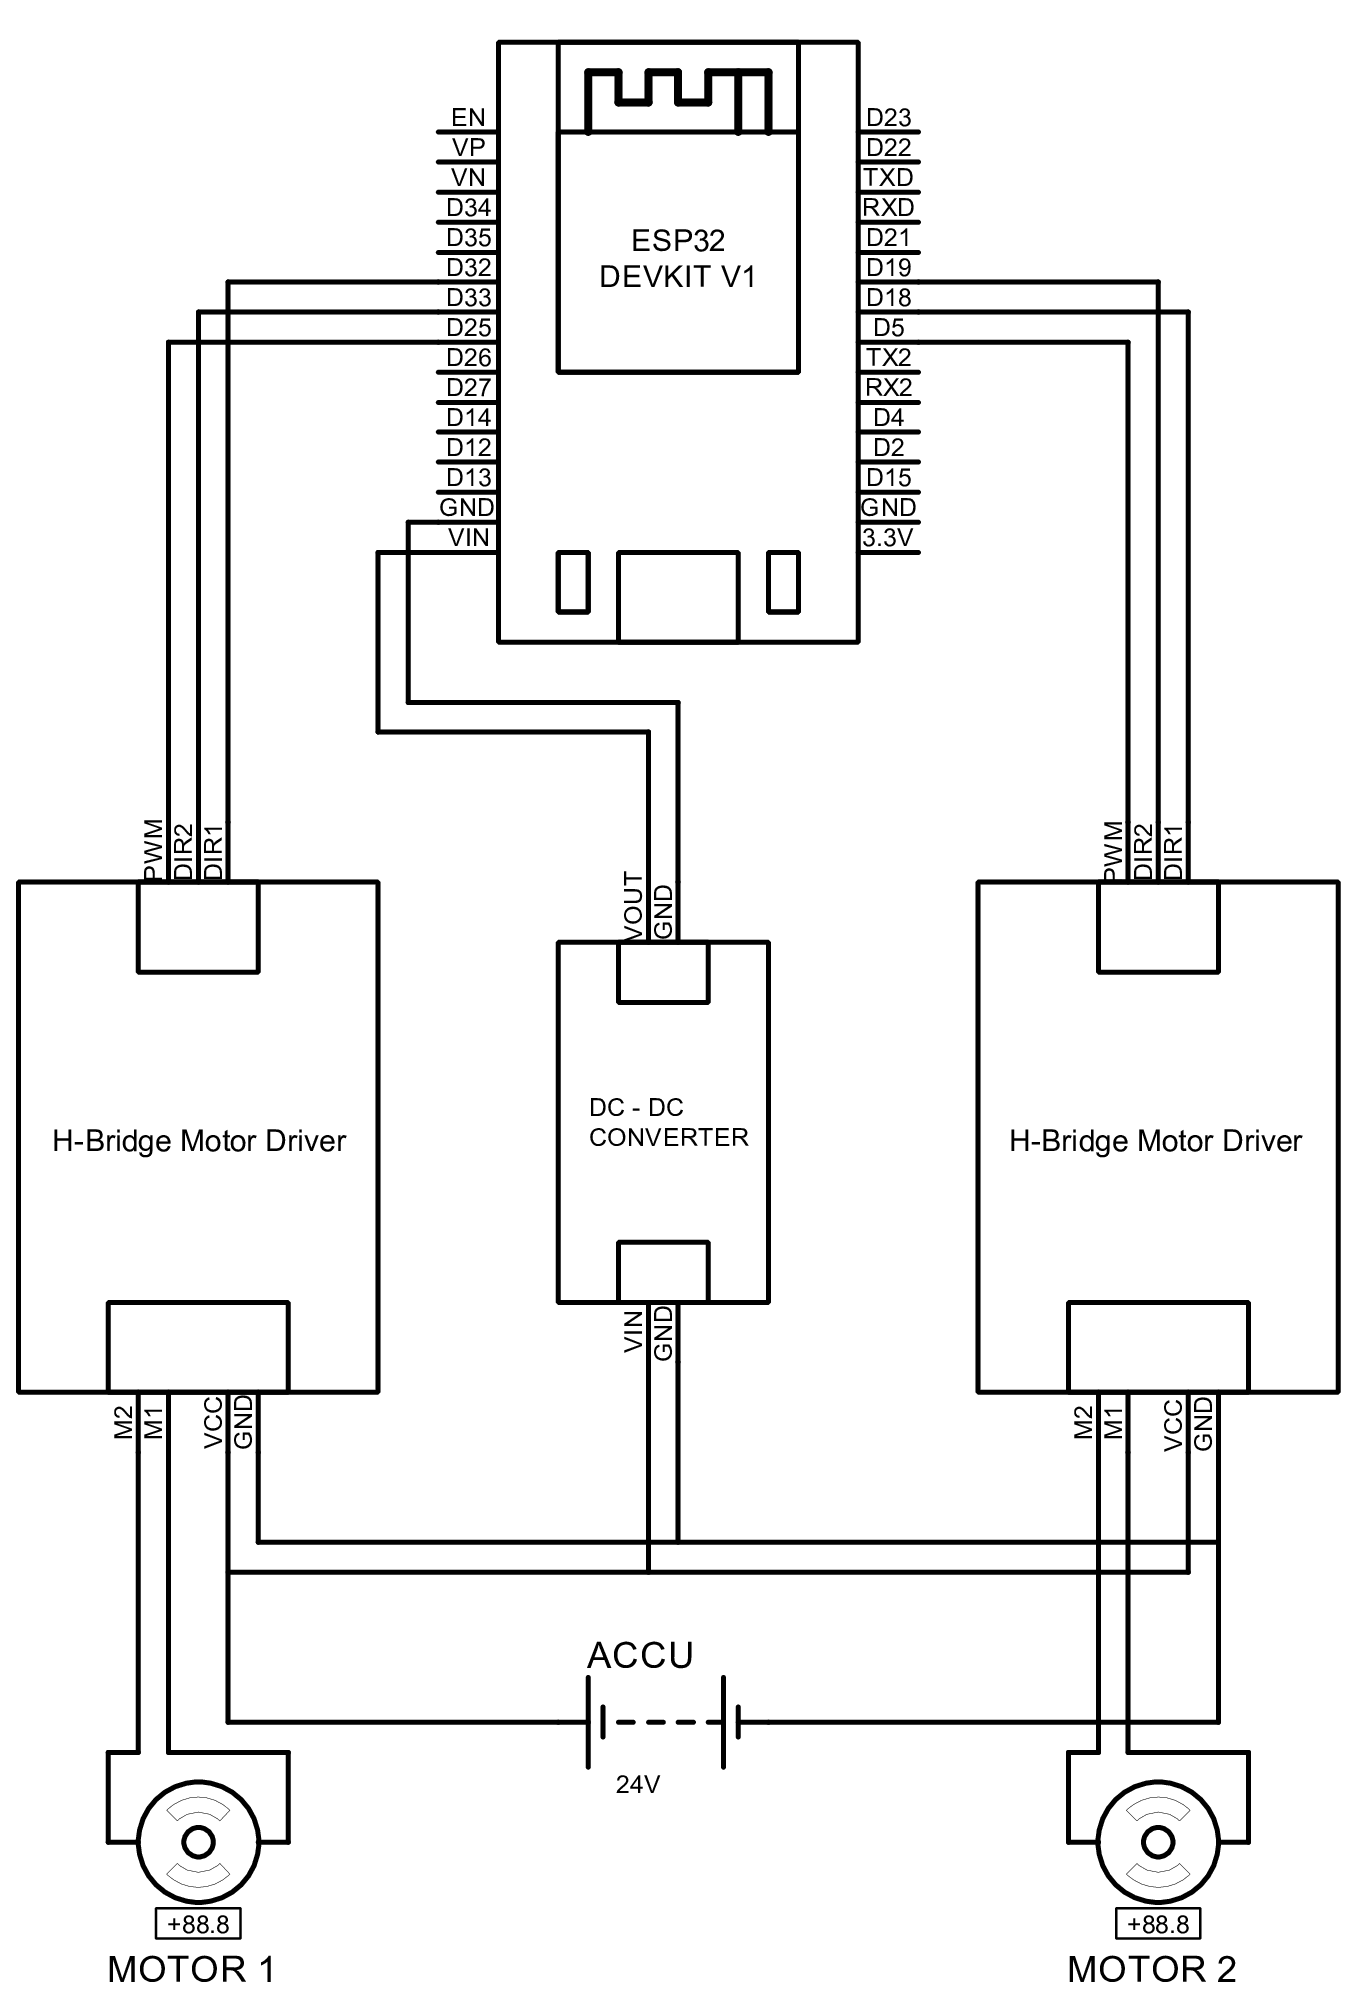
\includegraphics[scale=0.24]{gambar/bab3/Schematics.png}
  % Keterangan gambar yang diinputkan
  \caption{Schematic of the wheelchair motor control}
  % Label referensi dari gambar yang diinputkan
  \label{fig:Skematik Alat}
\end{figure}


  % Ubah judul dan label berikut sesuai dengan yang diinginkan.
\section{Lorem ipsum}
\label{sec:loremipsum}

% Ubah paragraf-paragraf pada bagian ini sesuai dengan yang diinginkan.

% Contoh input beberapa gambar pada halaman.
\begin{figure*}
  \centering
  \subfloat[Hasil A]{\includegraphics[width=.4\textwidth]{example-image-a}
    \label{fig:hasila}}
  \hfil
  \subfloat[Hasil B]{\includegraphics[width=.4\textwidth]{example-image-b}
    \label{fig:hasilb}}
  \caption{Contoh input beberapa gambar.}
  \label{fig:hasil}
\end{figure*}

\lipsum[16-18]

% Contoh input potongan kode dari file.
\lstinputlisting[
  language=Python,
  caption={Program perhitungan bilangan prima.},
  label={lst:bilanganprima}
]{program/bilangan-prima.py}

\lipsum[19-20]

  % Ubah judul dan label berikut sesuai dengan yang diinginkan.
\section{Kesimpulan}
\label{sec:kesimpulan}

% Ubah paragraf-paragraf pada bagian ini sesuai dengan yang diinginkan.
Berdasarkan hasil pengujian yang dilakukan selama pelaksanaan tugas akhir ini adalah sebagai berikut:

\begin{enumerate}

  \item Waktu \emph{delay} rata-rata terendah terdapat pada pengujian dengan mengirimkan string dengan 1 nilai dan ditransmisikan melalui WiFi. Waktu \emph{delay} rata-ratanya adalah sebesar 0,03499708571 detik.

  \item Waktu \emph{delay} rata-rata tertinggi terdapat pada pengujian dengan mengirimkan string dengan 2 nilai dan ditransmisikan melalui WiFi. Waktu \emph{delay} rata-ratanya adalah sebesar 1,059681387 detik.
  
  \item Waktu \emph{delay} tambahan pada program pengirim data diperlukan untuk beberapa pengujian. Hal ini diakibatkan agar tidak terjadi penumpukan (\emph{flooding}) data yang dapat mengganggu kinerja dari ESP32.

  \item Terdapat beberapa pengujian yang memerlukan waktu \emph{delay} tambahan pada program pengirim data seperti pada pengiriman data String berisi 2 nilai melalui Bluetooth yang memerlukan waktu \emph{delay} tambahan sebesar 1,5 detik, pengiriman data JSON dengan 2 nilai melalui Bluetooth yang memerlukan waktu \emph{delay} tambahan sebesar 1,1 detik, pengiriman data String berisi 2 nilai melalui WiFi yang memerlukan waktu \emph{delay} tambahan sebesar 1,3 detik, pengiriman data JSON yang berisi 2 nilai melalui WiFi yang memerlukan waktu \emph{delay} tambahan sebesar 1,5 detik, pengiriman data JSON yang berisi 1 nilai melalui Bluetooth yang memerlukan waktu \emph{delay} tambahan sebesar 1 detik, pengiriman data JSON yang berisi 1 nilai melalui WiFi yang memerlukan waktu \emph{delay} tambahan sebesar 1,5 detik.
  
  \item Hanya 2 pengujian yang tidak memerlukan waktu \emph{delay} tambahan pada program pengirim data, yaitu pada pengiriman data String yang berisi 1 nilai melalui Bluetooth dan pengiriman data String yang berisi 1 nilai melalui WiFi. 
  
  \item Data yang ditransmisikan untuk mengontrol kursi roda melalui visi komputer lebih baik menggunakan String yang hanya berisi 1 nilai, yaitu variabel arah yang dianalogikan dengan 1 karakter huruf. 
  
  \item Transmisi data yang digunakan untuk mengontrol kursi roda melalui visi komputer lebih baik menggunakan WiFi dengan ESP32 sebagai \emph{Access Point}-nya.

\end{enumerate}

\section{Saran}
\label{chap:saran}

Berdasarkan hasil yang diperoleh dari penelitian ini maka saran yang dapat dipertimbangkan untuk pengembangan lebih lanjut adalah sebagai berikut:

\begin{enumerate}

  \item Kecepatan putar motor diatur melalui ESP32 dengan menggunakan \emph{button} ataupun potensiometer.

  \item Mencoba menggunakan gestur lain untuk mengontrol gerak kursi roda.

\end{enumerate}


  % Menampilkan daftar pustaka dengan format IEEE
  \bibliographystyle{IEEEtranN}
  \bibliography{pustaka/pustaka.bib}

  % Menyeimbangkan bagian akhir di kedua kolom
  \balance

\end{document}
